\documentclass{article}

\usepackage{multicol}
\usepackage{geometry}
\usepackage{blindtext}
\usepackage[T1]{fontenc}
\usepackage{graphicx}
\usepackage{pdfpages}

\geometry{
  a4paper,
  left=20mm,
  right=20mm,
  top=20mm,
  bottom=20mm
}

\renewcommand{\tablename}{Tabla}

\title{Proyecto de ciencia de datos reproducible}
\author{Lluís Baldirà Jorro}
\date{\today}

\usepackage{Sweave}
\begin{document}
\Sconcordance{concordance:Knitr_informe.tex:Knitr_informe.Rnw:1 23 1 1 0 18 1 1 8 24 %
1 1 49 14 0 1 2 2 0 1 1 4 0 1 2 4 1 1 5 1 1 1 57 7 1 1 40 1 1 1 5 9 1 1 %
60 18 1}



\maketitle

\section*{Datos emociones positivas y negativas}
\textbf{En el presente documento se lleva a cabo un estudio para observar los diferentes niveles de emociones positivas y negativas a lo largo de tres periodos anuales (2006, 2014 y 2023) para diferentes paises y edades. A continuación se mostraran los objetivos del proyecto y la definición de las variables con las que se va a trabajar:}
\subsection*{Objectivo principal}
\emph{Evaluar la evolución de las emociones positivas y negativas en diferentes países a lo largo del tiempo, analizando las diferencias entre grupos de edad y países, con el fin de identificar patrones y tendencias que puedan contribuir a una mejor comprensión del bienestar subjetivo a nivel internacional.}
\subsubsection*{Objetivos específicos}
\begin{itemize}
\item Caracterizar los niveles de felicidad, disfrute de vida, tristeza y depresión en cada país y periodo.
\item Explorar si existen patrones o tendencias en la evolución de las emociones a lo largo del tiempo (por ejemplo, aumento o disminución de la felicidad a lo largo de los 3 periodos).
\item Evaluar si la edad es un factor significativo en la experiencia emocional.
\item Analizar las diferencias en los niveles de emociones positivas y negativas entre países y grupos de edad.
\item Representar los resultados de manera clara y concisa utilizando gráficos y tablas
\end{itemize}



\section{Definición de las variables}
\begin{enumerate}
\item \underline{felicidad}: nivel de felicidad en la última semana, con 4 opciones de respuesta de 1 (None or almost none of the time) a 4 (All or almost all of the time).

\item \underline{disfrute de vida}: Nivel de disfrute de vida la ultima semana, con 4 opciones de respuesta de 1 (None or almost none of the time) a 4 (All or almost all of the time).

\item \underline{tristeza}: nivel de tristeza en la última semana, con 4 opciones de respuesta de 1 (None or almost none of the time) a 4 (All or almost all of the time).

\item \underline{depresion}: nivel de depresión en la última semana, con 4 opciones de respuesta de 1 (None or almost none of the time) a 4 (All or almost all of the time).

\item \underline{cntry}: País del participante de donde se ha sacado la observación.

\item \underline{año}: Año en que se ha obtenido la observación, pudiendo ser 2006, 2014 o 2023.

\item \underline{agea}: Edad del participante.

\end{enumerate}



\section{Tabla resumen de las variables}


\begin{Schunk}
\begin{Soutput}
                 vars     n  mean    sd median trimmed   mad min max range
felicidad           1 55962  2.97  0.78      3    3.01  0.00   1   4     3
disfrute_de_vida    2 55962  2.96  0.82      3    3.02  1.48   1   4     3
tristeza            3 55962  1.48  0.64      1    1.39  0.00   1   4     3
depresion           4 55962  1.41  0.64      1    1.29  0.00   1   4     3
agea                5 55962 49.66 18.65     50   49.56 22.24  14 104    90
                  skew kurtosis   se
felicidad        -0.43    -0.18 0.00
disfrute_de_vida -0.44    -0.38 0.00
tristeza          1.31     1.89 0.00
depresion         1.66     2.81 0.00
agea              0.04    -0.91 0.08
\end{Soutput}
\begin{Soutput}
Posibles valores de cntry:
\end{Soutput}
\begin{Soutput}
 [1] AT CH DE FI GB HU IE NL NO SI
Levels: AT CH DE FI GB HU IE NL NO SI
\end{Soutput}
\end{Schunk}


\section{Gráficos del proyecto}
\subsection{Gráficos de emociones por año}



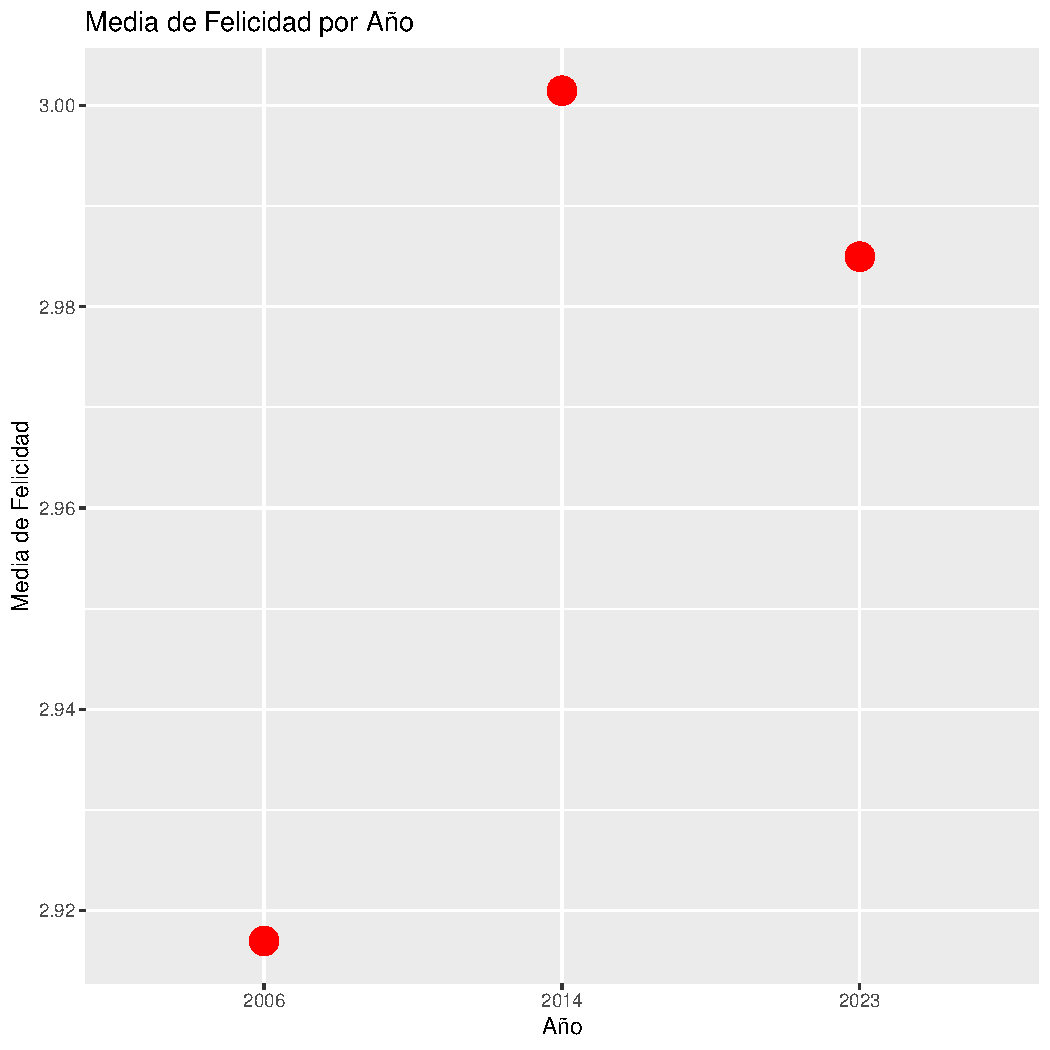
\includepdf[pages=1-4]{Rplots.pdf}




\subsection{Gráficos de emociones por país}







\includepdf[pages=5-14]{Rplots.pdf}



\subsection{Gráficos de emociones por edad}



\includepdf[pages=15-18]{Rplots.pdf}


\section*{Comentarios}
A primera vista, no se observan grandes diferencias en cuanto a la percepción de emociones positivas y negativas en función de la edad, a excepción de una ligera tendencia creciente en cuanto a depresión y tristeza entre los 75 y 90 años, volviendo a decaer después de esa franja. En cuanto a los paises tampoco se aprecian grandes diferencias, todos se mantienen en un rango similar, y a nivel global destacar que en 2014 se encontramos los picos de mayor valor para las emociones positivas, y de menor valor para las emociones negativas, cambiando la tendencia de 2006 a 2023, aunque estos cambios no parecen muy significativos pues los valores medios varian entre 0.1 y 0.05.












\end{document}
